\documentclass{beamer}

\usepackage{multirow}
\usepackage{pgfpages}
%\setbeameroption{show notes}
%\setbeameroption{show notes on second screen=right}
\mode<presentation> {
  \usetheme{Warsaw}
  \setbeamercovered{transparent}
}
\usepackage{graphicx}
\usepackage[english]{babel}
\usepackage[utf8]{inputenc}
\usepackage{times}
\usepackage[T1]{fontenc}
\usepackage{colortbl}
\usepackage{tikz}
\usepackage{pbox}
\usepackage{tcolorbox}

%\pgfdeclareimage[height=0.5cm]{le-logo}{logo-irisa}
%\logo{\pgfuseimage{le-logo}}

\setbeamertemplate{headline}{}
\setbeamertemplate{footline}[]

\AtBeginSection[]{
  \begin{frame}
  \vfill
  \centering
  \begin{beamercolorbox}[sep=8pt,center,shadow=true,rounded=true]{title}
    \usebeamerfont{title}\insertsectionhead\par%
  \end{beamercolorbox}
  \vfill
  \end{frame}
}

%%%%%%%%%%%%%%%%%%%%%%%%%%%
\title[] 
{Scalable Models of Probabilistic Forecasting with Fuzzy Time Series}
%\subtitle {}

\author[] {Petrônio C. L. Silva}


\institute[]
{
  Graduate Program in Electrical Engineering - PPGEE\\
  Federal University of Minas Gerais - UFMG, Belo Horizonte, MG, Brazil\\
  Machine Intelligence and Data Science (MINDS) Lab\\
}


\date[Belo Horizonte, 2019] 

\begin{document}
\newcommand{\var}{\mathcal{V}}
\newcommand{\vari}{\mathcal{V}_i}
\newcommand{\ulvar}{\tilde{A}}
\newcommand{\mlvar}{\widetilde{\mathcal{V}}_i}
\newcommand{\tlvar}{\widetilde{*\mathcal{V}}}
\newcommand{\ufset}{A_j}
\newcommand{\mfset}{A_j^{\vari}}
\newcommand{\tfset}{A_j^{*\var}}
\newcommand{\model}{\mathcal{M}}
\newcommand{\estimate}{\hat{y}(t+1)}
\newcommand{\intvl}{\mathbb{I}}
\newcommand{\interval}{\intvl = [\underline{l},\overline{u}{]}}
\newcommand{\ifts}{[\mathbb{I}]FTS}
\newcommand{\FIG}{\mathcal{FIG}}
\newcommand{\fig}{\mathcal{G}}
\newcommand{\figi}{\mathcal{G}_i}
\renewcommand{\textdegree}{$^{\circ}$}


\beamertemplatenavigationsymbolsempty
\linespread{1.0}

%%%%%%%%%%%%%%%%%%%%%%%%%%%%%%%%%%%%%%%%%%%%%%

\begin{frame}
  \titlepage
\end{frame}

%%%%%%%%%%%%%%%%%%%%%%%%%%%%%%%%%%%%%%%%%%%%%%

\begin{frame}{Schedule}
  \tableofcontents
\end{frame}

%%%%%%%%%%%%%%%%%%%%%%%%%%%%%%%%%%%%%%%%%%%%%%
%%%%%%%%%%%%%%%%%%%%%%%%%%%%%%%%%%%%%%%%%%%%%%

\section{Introduction}

%%%%%%%%%%%%%%%%%%%%%%%%%%%%%%%%%%%%%%%%%%%%%%

\begin{frame}{Introduction - Scenario}
\linespread{2}
\begin{itemize}
\item Smart Grids and Environments
\begin{itemize}
\item Ubiquitous Computing;
\begin{itemize}
\item Smart sensors, stream data w/ high sampling rate 
\end{itemize}
\item Integration with Renewable Energy;
\begin{itemize}
    \item Non perennial, less reliable 
\end{itemize}
\item Intelligent Management;
\begin{itemize}
    \item Forecasting for dynamic optimization
\end{itemize}
\end{itemize}
\end{itemize}
\end{frame}

\note[itemize]{
\item Intelligent Management = Dynamic Robust Optimization
}

%%%%%%%%%%%%%%%%%%%%%%%%%%%%%%%%%%%%%%%%%%%%%%

\begin{frame}{Introduction - Demands}
\linespread{1.5}
\begin{itemize}
\item Accurate forecasting of complex multivariate stochastic processes;
\item Big Data:
\begin{itemize}
    \item Storage and processing issues;
\end{itemize}
\item Regulatory barriers;
\begin{itemize}
    \item Auditability? 
\end{itemize}
\end{itemize}
\end{frame}

%%%%%%%%%%%%%%%%%%%%%%%%%%%%%%%%%%%%%%%%%%%%%%

\begin{frame}{Introduction - Opportunity}
\linespread{2}
\begin{itemize}
\item Fuzzy Time Series
\begin{itemize}
\item Accurate and computationally cheap
\item White box methods;
\begin{itemize}
    \item human-readable and auditable models
\end{itemize}
\item Data Driven / Non Parametric
\item Flexibility
\end{itemize}
\end{itemize}
\end{frame}



%%%%%%%%%%%%%%%%%%%%%%%%%%%%%%%%%%%%%%%%%%%%%%

\begin{frame}{Objectives}
\linespread{2}
\begin{itemize}
\item This works aims to:
\begin{enumerate}
\item Introduce the Weighted Multivariate FTS (WMVFTS), a new forecasting approach for multivariate time series using Fuzzy Time Series;
\item Extend the sequential WMVFTS method to a distributed design using Map/Reduce paradigm;
\item Use the proposed methods to tackle a big environmental time series focused on renewable energy forecasting;
\end{enumerate}
\end{itemize}
\end{frame}

%%%%%%%%%%%%%%%%%%%%%%%%%%%%%%%%%%%%%%%%%%%%%%
%%%%%%%%%%%%%%%%%%%%%%%%%%%%%%%%%%%%%%%%%%%%%%

\section{Literature Review}

%%%%%%%%%%%%%%%%%%%%%%%%%%%%%%%%%%%%%%%%%%%%%%

\begin{frame}{Literature Review - Fuzzy Time Series Models}

\begin{itemize}
\item Proposed in \cite{song1993fuzzy}
\item Application fields
\begin{itemize}
\item Energy load  \cite{Sadaei2017, Severiano2017a, Silva2017a, Silva2018a}
\item Stock index prices \cite{Sadaei2016, Silva2016ifts,Talarposhti2016a}
\item Interval and probabilistic \cite{Silva2016ifts, Alves2018}
\end{itemize}
\end{itemize}
\end{frame}

\note[itemize]{
\item 
}

%%%%%%%%%%%%%%%%%%%%%%%%%%%%%%%%%%%%%%%%%%%%%%

\begin{frame}{Literature Review - Fuzzy Time Series Models}
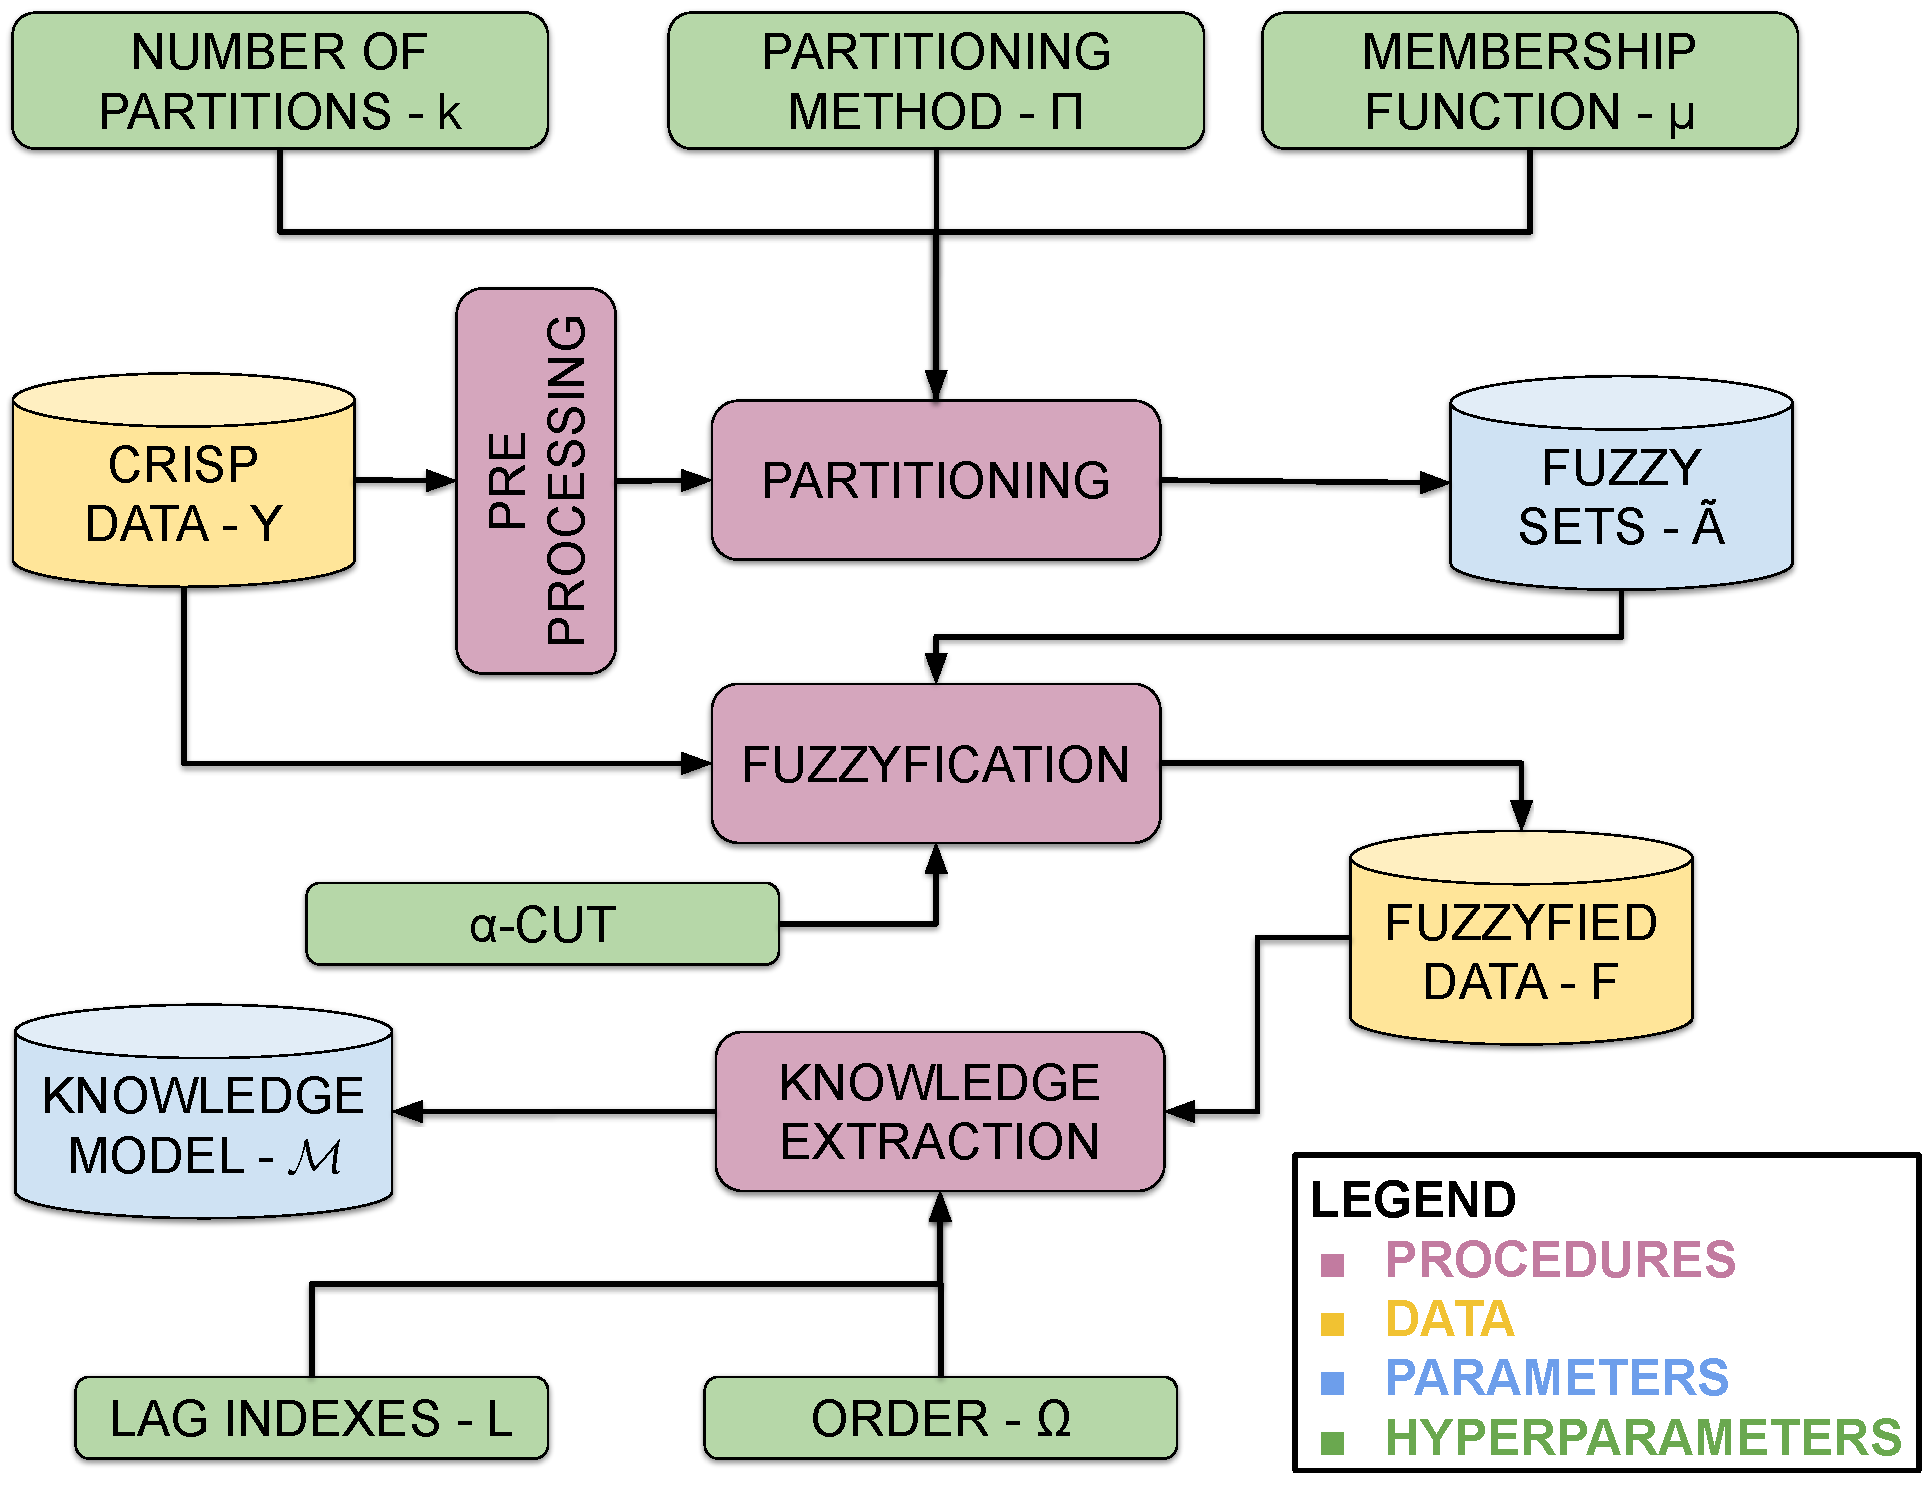
\includegraphics[width=\textwidth,height=8cm]{figures/fts_training.pdf}
\end{frame}

%%%%%%%%%%%%%%%%%%%%%%%%%%%%%%%%%%%%%%%%%%%%%%

\begin{frame}{Literature Review - Fuzzy Time Series Models}
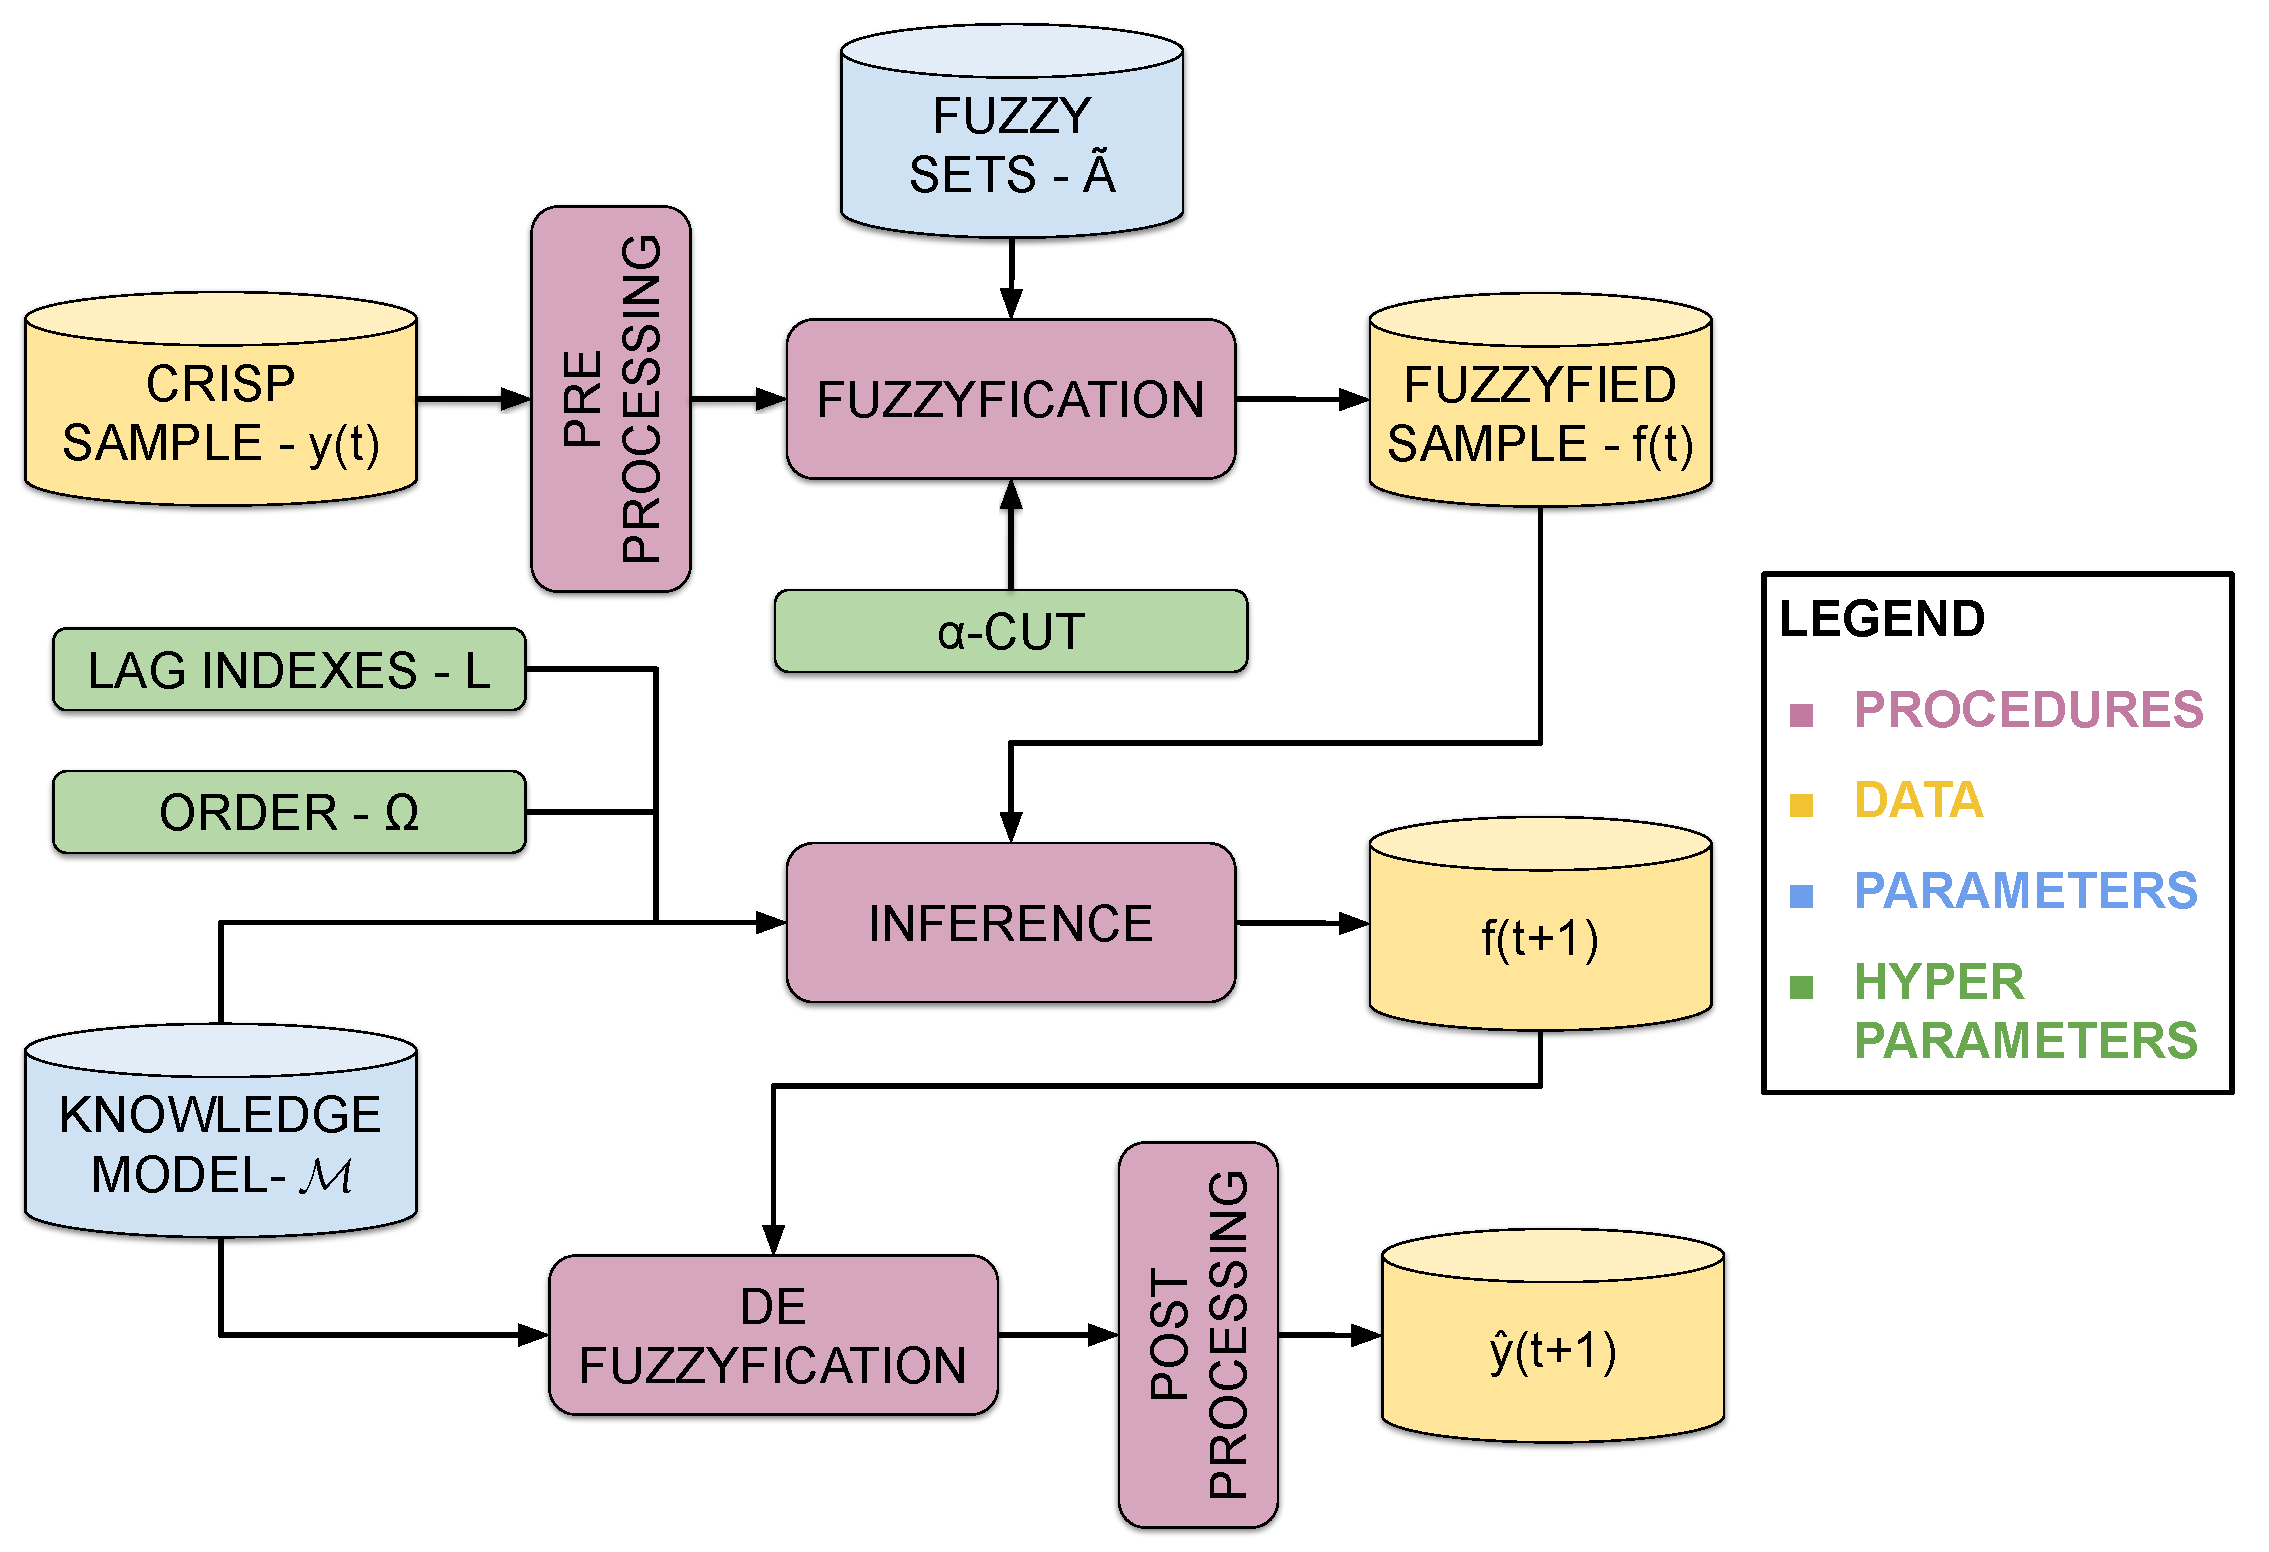
\includegraphics[width=\textwidth,height=8cm]{figures/fts_forecasting.pdf}
\end{frame}


%%%%%%%%%%%%%%%%%%%%%%%%%%%%%%%%%%%%%%%%%%%%%%

\begin{frame}{Literature Review}
\linespread{2}
\begin{itemize}
\item Map/Reduce paradigm\cite{Dean2008}
\begin{itemize}
    \item SIMD - Single Instruction Multiple Data
    \item Master-Slave architecture
\end{itemize}
\item Apache Hadoop\cite{White2012}
\item Apache Spark
\end{itemize}
\end{frame}

\note[itemize]{
\item 
}

%%%%%%%%%%%%%%%%%%%%%%%%%%%%%%%%%%%%%%%%%%%%%%

\begin{frame}{Literature Review}

\begin{figure}
    \centering
    \includegraphics[width=\textwidth,height=7cm]{figures/mapreduce.png}
    \caption{Map/Reduce Paradigm \cite{Dean2008}}
    \label{fig:my_label}
\end{figure}

\end{frame}

\note[itemize]{
\item For algorithms that can be decomposed in small jobs, whose results can be aggregated 
}

%%%%%%%%%%%%%%%%%%%%%%%%%%%%%%%%%%%%%%%%%%%%%%

\begin{frame}{Literature Review}

\begin{figure}
    \centering
    \includegraphics[width=\textwidth,height=7cm]{figures/hadoop_cluster.png}
    \caption{Hadoop Cluster}
    \label{fig:my_label}
\end{figure}

\end{frame}

\note[itemize]{
\item A key feature of this architecture is the possibility to create powerful storage and processing platforms using cheap and commodity hardware.
}

%%%%%%%%%%%%%%%%%%%%%%%%%%%%%%%%%%%%%%%%%%%%%%
%%%%%%%%%%%%%%%%%%%%%%%%%%%%%%%%%%%%%%%%%%%%%%
\section{Weighted Multivariate Fuzzy Time Series - WMVFTS}

%%%%%%%%%%%%%%%%%%%%%%%%%%%%%%%%%%%%%%%%%%%%%%
\begin{frame}{Definitions and notations}
\begin{table}[]
    \centering
    \begin{tabular}{|c|m{7cm}|} \hline
        $Y \in \mathbb{R}^n$ &  the multivariate time series \\ \hline
        $n = |\var|$ & the number of variables of $Y$  \\ \hline
        $y(t) \in Y$ & an individual instance of $Y$ \\ \hline
        $T \in \mathbb{R}^1$ & the total length of $Y$ \\ \hline
        $t \in T$ & the time index \\ \hline
        $\var$ & the set of variables of $Y$ \\ \hline
        $\vari \in \var$ & an individual variable \\ \hline
        $U_i$ & the Universe of Discourse of each  $\vari$ \\ \hline
        $*\var \in \var$ & the target variable \\ \hline
        $\lvar$ & the linguistic variable, the group of fuzzy sets created for each $\vari$ \\ \hline
        $\fset \in \lvar$ & the individuals fuzzy sets in $\lvar$ \\ \hline
    \end{tabular}
    \caption{Notations and its definitions}
    \label{tab:my_label}
\end{table}
\end{frame}

%%%%%%%%%%%%%%%%%%%%%%%%%%%%%%%%%%%%%%%%%%%%%%
\begin{frame}{Sequential WMVFTS}
\begin{itemize}
\item MISO: Multiple Input Single Output
\item $n-1$ explanatory variables $\vari \in \var$
\item One target variable $*\var \in \var$
\end{itemize}
\end{frame}

%%%%%%%%%%%%%%%%%%%%%%%%%%%%%%%%%%%%%%%%%%%%%%
\begin{frame}{Sequential WMVFTS - Training Procedure}
\centering
\includegraphics[width=\textwidth]{figures/training_process.pdf}
\end{frame}

%%%%%%%%%%%%%%%%%%%%%%%%%%%%%%%%%%%%%%%%%%%%%%
\begin{frame}{Sequential WMVFTS - Training Procedure}
\begin{table}[]
    \centering
    \begin{tabular}{|c|m{6cm}|} \hline
        \textbf{Alias} & \textbf{Parameter} \\ \hline
         $k_i \in \mathbb{N}^+$ & Number of partitions (fuzzy sets) \\ \hline
         $\mu_i: U_i \rightarrow [0,1] $ & Membership function, measures the membership of a value $y \in U$ to a fuzzy set  \\\hline
         $\alpha_i \in [0,1]$ & the $\alpha$-cut, the minimal membership grade to take account on fuzzyfication process \\ \hline
    \end{tabular}
    \caption{WMVFTS hyperparameters for each variable $\vari \in \var$}
    \label{tab:hyperparameters}
\end{table}
\end{frame}

%%%%%%%%%%%%%%%%%%%%%%%%%%%%%%%%%%%%%%%%%%%%%%
\begin{frame}{Sequential WMVFTS }
\linespread{2}
\begin{enumerate}
\item[Stage 1] \textit{Partitioning}:
\begin{enumerate}
\item \textit{Defining $U_{\vari}$}: $U_{\vari} = [\min(Y^{\vari})-D_1, \max(Y^{\vari})+D_2]$, 
$D_1 = \min(Y^{\vari})\times 0.2$
$D_2 = \max(Y^{\vari})\times 0.2$ 

\item \textit{$U_{\vari}$ Partitioning}: Split $U_{\vari}$ in $k_i$ intervals $U_j$;

\item \textit{Define the linguistic variable $\lvar$}:  $\forall U_j \in U_{\vari}$  create a fuzzy set $\fset$, with the membership function $\mu_{\fset}$. 
\end{enumerate}
\end{enumerate}
\end{frame}

%%%%%%%%%%%%%%%%%%%%%%%%%%%%%%%%%%%%%%%%%%%%%%
\begin{frame}{Sequential WMVFTS }
\linespread{2}
\begin{enumerate}
\item[Stage 2] \textit{Fuzzyfication}: 
\begin{itemize}
    \item Transform the original numeric time series $Y$ into a fuzzy time series $F$
    \item $\forall y(t) \in Y$:
    \begin{itemize}
    \item $f(t) = \{\fset\; |\; \mu_{\fset}(y(t)^{\vari}) \geq \alpha_i\;\;\forall \fset \in \lvar\}$
    \end{itemize}
\end{itemize}
\end{enumerate}
\end{frame}

%%%%%%%%%%%%%%%%%%%%%%%%%%%%%%%%%%%%%%%%%%%%%%
\begin{frame}{Sequential WMVFTS }
\linespread{1}
\begin{enumerate}
\item[Stage 3] \textit{Rule Induction}: 
\begin{enumerate}
\item \textit{Generate the temporal patterns}:  

$A_j^{\var_0},...,A_j^{\var_n} \rightarrow A_j^{*\var}$
where $f(t) = \fset, \forall \vari \in \var$ and $f(t+1) = \tfset$, $\tfset \in \tlvar$.

\item \textit{Generate the rule base $\mathcal{M}$}: 
$\var \rightarrow w_k \cdot A_k^{*\var}, w_j \cdot A_j^{*\var},...$, where the LHS is $f(t) = \fset, \forall \vari \in \var$ and the RHS is $f(t+1) \in \{A_k^{*\var},A_j^{*\var},... \}$ 
\begin{equation}
w_i = \frac{\#\tfset}{\#RHS} \quad \forall \tfset \in RHS    
\end{equation}
\end{enumerate}
\end{enumerate}
\end{frame}

%%%%%%%%%%%%%%%%%%%%%%%%%%%%%%%%%%%%%%%%%%%%%%
\begin{frame}{Sequential WMVFTS - Model}
$$
\var \rightarrow w_k \cdot A_k^{*\var}, w_j \cdot A_j^{*\var},...
$$
\end{frame}


%%%%%%%%%%%%%%%%%%%%%%%%%%%%%%%%%%%%%%%%%%%%%%
\begin{frame}{Sequential WMVFTS - Forecasting Procedure}
\centering
\includegraphics[width=\textwidth]{figures/forecasting_process.pdf}
\end{frame}

%%%%%%%%%%%%%%%%%%%%%%%%%%%%%%%%%%%%%%%%%%%%%%
\begin{frame}{Sequential WMVFTS - Forecasting Procedure}
\begin{enumerate}
\item [Step 1] \textit{Fuzzyfication}:
\begin{equation}
f(t) = \{\fset\; |\; \mu_{\fset}(y(t)^{\vari}) \geq \alpha_i\;\;\forall \fset \in \lvar\}
\end{equation}
\item [Step 2] \textit{Rule matching}: 
\begin{equation}
    active\_rules = \{ f(t) = rule_{precedent} | \forall rule \in \mathcal{M} \}
\end{equation}
\begin{equation}
    \mu_{rule} = \bigcap_{j \in f(t)} \mu_{\fset}(y(t))
\end{equation}
\item [Step 3] \textit{Defuzzyfication}:
\begin{equation}
midpoint_{rule} = \sum_{j \in *\lvar} w_j \cdot c_j
\end{equation}
\begin{equation}
\hat{y}(t+1) = \frac{\sum_{rule \in active\_rules} \mu_{rule} \cdot midpoint_{rule}}{\sum_{rule \in active\_rules} \mu_{rule}}
\end{equation}
\end{enumerate}
\end{frame}

%%%%%%%%%%%%%%%%%%%%%%%%%%%%%%%%%%%%%%%%%%%%%%
\begin{frame}{Distributed WMVFTS - Core Ideas}
\begin{itemize}
    \item A huge time series $Y$ can be sliced in smaller ones;
    \item WMVFTS models can be trained with these slices;
    \item The rules of the different models can be merged;
    \item The weights just need to be recalculated;
\end{itemize}
\end{frame}

%%%%%%%%%%%%%%%%%%%%%%%%%%%%%%%%%%%%%%%%%%%%%%
\begin{frame}{Distributed WMVFTS - Training Procedure}
\centering
\includegraphics[width=\textwidth,height=7cm]{figures/distributed_training.pdf}
\end{frame}

%%%%%%%%%%%%%%%%%%%%%%%%%%%%%%%%%%%%%%%%%%%%%%
\begin{frame}{Distributed WMVFTS - Training Procedure}
\textbf{Partitioning}:
    \begin{enumerate}
        \item \textbf{Share}: $k_i$,$\mu_i$; 
        \item \textbf{Map}: Distribute the $Y$ and return $U_{\vari}^p$;
        \item \textbf{Reduce}: Collect the $U_{\vari}^p$, and generate $U_{\vari} = \bigcup U_{\vari}^p$;
        \item \textbf{Create}: Proceed the sequential partitioning, creating the linguistic variables $\lvar$. 
    \end{enumerate}
\end{frame}

%%%%%%%%%%%%%%%%%%%%%%%%%%%%%%%%%%%%%%%%%%%%%%
\begin{frame}{Distributed WMVFTS - Training Procedure}
\textbf{Fuzzyfication \& Rule Induction}:
    \begin{enumerate}
        \item \textbf{Share}: $\lvar$, $*\var$, $\alpha_i \forall\vari \in \var$;
        \item \textbf{Map}: Distribute the $Y$, returning the local WMVFTS models $\mathcal{M}_p$; 
        \item \textbf{Reduce}: Collect all $\mathcal{M}_p$ models; 
        \item \textbf{Merge}: $\mathcal{M} = \bigcup \mathcal{M}_p$
    \end{enumerate}
\end{frame}

%%%%%%%%%%%%%%%%%%%%%%%%%%%%%%%%%%%%%%%%%%%%%%
\begin{frame}{Distributed WMVFTS - Training Procedure}
\begin{itemize}
    \item $\mathcal{M} = \bigcup \mathcal{M}_p$ 
    \item For each rule $LHS \rightarrow RHS$ in all collected models $\mathcal{M}_p$:
        \begin{enumerate}
            \item If $\mathcal{M}$ does not contain the $LHS$, then append the entire rule on $\mathcal{M}$;
            \item If $\mathcal{M}$ contains the $LHS$, then for each $w_j \cdot \tfset \in RHS$:
            \begin{enumerate}
            \item If the $RHS$ on $\mathcal{M}$ does not contain $\tfset$, then append $w_j \cdot \tfset$ on $RHS$ and add $w_j$ on $\#RHS$
            \item If the $RHS$ on $\mathcal{M}$ contains $\tfset$, then add $w_j$ on existing weight and add $w_j$ on $\#RHS$
            \end{enumerate}
            \end{enumerate}
\end{itemize}
\end{frame}


%%%%%%%%%%%%%%%%%%%%%%%%%%%%%%%%%%%%%%%%%%%%%%
%%%%%%%%%%%%%%%%%%%%%%%%%%%%%%%%%%%%%%%%%%%%%%
\section{Computational Experiments}

%%%%%%%%%%%%%%%%%%%%%%%%%%%%%%%%%%%%%%%%%%%%%%
\begin{frame}{Computational Experiments - Technologies}
\begin{center}
    \begin{tabular}{cc}
        \includegraphics[height=2cm]{figures/python.jpg} 
        &
        \includegraphics[height=2.5cm]{figures/pyFTS.png}
        \\
        &
        \\
        \includegraphics[width=4cm, height=2cm]{figures/hadoop.png}
         & 
         \includegraphics[width=3cm, height=2cm]{figures/spark.png}
    \end{tabular}
\end{center}
\end{frame}

%%%%%%%%%%%%%%%%%%%%%%%%%%%%%%%%%%%%%%%%%%%%%%
\begin{frame}{Computational Experiments - Dataset}
\linespread{1.5}
\begin{itemize}
\item SONDA - System of National Organization of Environmental Data\footnote{\url{http://sonda.ccst.inpe.br/}} from Brazilian Spatial Research Institute (INPE);
\item Global Solar Radiation from Brasília\footnote{Code: BRB. Coordinates: 15\textdegree 36' 03" S 47\textdegree 42'47" O. Alt.: 1023m} meteorological station;
\item Recorded between 2012 and 2015, by minute;
\item 2 million instances.
\end{itemize}
\end{frame}

%%%%%%%%%%%%%%%%%%%%%%%%%%%%%%%%%%%%%%%%%%%%%%
\begin{frame}{Computational Experiments - Dataset}
\centering
\includegraphics[width=\textwidth]{figures/sonda_sample.png}
\end{frame}

%%%%%%%%%%%%%%%%%%%%%%%%%%%%%%%%%%%%%%%%%%%%%%
\begin{frame}{Computational Experiments - Grid Search}

\begin{table}
    \centering
    \begin{tabular}{|c|c|} \hline
        \textbf{Parameter} & \textbf{Search Space} \\ \hline
         $k$ & $[10,100]$ \\ \hline
         $\mu$ & triangular, trapezoidal, gaussian  \\ \hline
         $\alpha$ & $\{0, .05, .15, .2, .25, .3,  .35, .4, .45, .5\}$  \\ \hline
    \end{tabular}
    \caption{Hyper-parameters search spaces for each variable}
    \label{tab:hyperparam_const}
\end{table}

\begin{itemize}
    \item Computational cluster:
    \begin{itemize}
        \item Number of nodes: [1, 9]
        \item Heterogeneous machines on a 100mbps LAN
        \item Commodity cheap hardware
    \end{itemize}
\end{itemize}

\end{frame}

%%%%%%%%%%%%%%%%%%%%%%%%%%%%%%%%%%%%%%%%%%%%%%
\begin{frame}{Computational Experiments - Results}

\begin{figure}
    \includegraphics[width=\textwidth, height=3.5cm]{figures/training.png}
    %\caption{Training speed up}
\end{figure}

\begin{table}[]
    \centering
    \begin{tabular}{|c|c|c|}
\hline
\multirow{2}{*}{\textbf{Cores}} & \multicolumn{2}{c|}{\textbf{Training}} \\ \cline{2-3} 
& \textbf{Time}    & \textbf{Speed Up}    \\ \hline
1 & $693.41 \pm 11.05$ & -     \\ \hline
3 & $746.15 \pm 29.30$ & $0.92 \pm	0.03$ \\ \hline
5 & $508.75 \pm 12.21$ & $1.35 \pm	0.03$ \\ \hline
7 & $455.25 \pm	7.98$ & $1.51 \pm 0.02$  \\ \hline
9 & $414.25 \pm	8.16$ & $1.66 \pm 0.03$ \\ \hline
\end{tabular}
\end{table}

\end{frame}



%%%%%%%%%%%%%%%%%%%%%%%%%%%%%%%%%%%%%%%%%%%%%%
\begin{frame}{Computational Experiments - Results}
\linespread{1}
\begin{figure}
    \includegraphics[width=\textwidth, height=3.5cm]{figures/forecasting.png}
    %\caption{Forecasting speed up}
\end{figure}
\begin{table}[]
    \centering
    \begin{tabular}{|c|c|c|}
\hline
\multirow{2}{*}{\textbf{Cores}} & \multicolumn{2}{c|}{\textbf{Forecasting}} \\ \cline{2-3} 
& \textbf{Time}    & \textbf{Speed Up}    \\ \hline
1 & - \\ \hline
3 & $246.25 \pm 10.82$ & $0.94 \pm 0.04$ \\ \hline
5 & $200.50 \pm 6.34$ & $1.15 \pm 0.03$ \\ \hline
7 & $181.75 \pm 5.06$ & $1.27 \pm 0.03$ \\ \hline
9 & $176.00 \pm 3.93$ & $1.31 \pm 0.02$ \\ \hline
\end{tabular}
\end{table}

\end{frame}

%%%%%%%%%%%%%%%%%%%%%%%%%%%%%%%%%%%%%%%%%%%%%%
\begin{frame}{Computational Experiments}
    \begin{table}[htb]
    \centering
    \begin{tabular}{|c|c|c|c|} \hline
        \textbf{Parameter} & \textbf{Month} & \textbf{Hour} & \textbf{Radiation} \\ \hline
         $k$ & $12$ & $24$ & $35$ \\ \hline
         $\mu$ & Triangular  & Triangular  & Triangular   \\ \hline
         $\alpha$ & $0.15$ & $0.15$ & $0.25$  \\ \hline
    \end{tabular}
    \caption{Best hyper-parameters found on Grid Search}
    \label{tab:results}
\end{table}
\end{frame}

%%%%%%%%%%%%%%%%%%%%%%%%%%%%%%%%%%%%%%%%%%%%%%
\begin{frame}{Computational Experiments}

\includegraphics[width=\textwidth, height=8cm]{figures/variables.png}

\end{frame}


\note[itemize]{
\item 
}

%%%%%%%%%%%%%%%%%%%%%%%%%%%%%%%%%%%%%%%%%%%%%%
\begin{frame}{Computational Experiments}
\begin{table}[]
    \centering
    \begin{tabular}{ccc}
    Dec,14hs,R29 & $\rightarrow$ & (.2) R28, (.45) R29, (.35) R30  \\
    & & \\
    Dec,15hs,R29 & $\rightarrow$ & (.1) R28, (.4) R29, (.4) R30, (.1) R31  \\
    & & \\
    Jan,14hs,R30 & $\rightarrow$ & (.1) R29, (.5) R30, (.25) R31, (.15) R32  \\
    & & \\
    Jan,15hs,R30 & $\rightarrow$ & (.3) R30, (.35) R31, (.35) R32
    & & \\
    Fev,14hs,R31 & $\rightarrow$ & (.30) R30, (.45) R31, (.25) R32  \\
    & & \\
    Fev,15hs,R31 & $\rightarrow$ & (.30) R30, (.35) R31, (.35) R32  \\
    \end{tabular}
    \caption{Sample of generated rules}
    \label{tab:my_label}
\end{table}

\end{frame}


\note[itemize]{
\item 
}

%%%%%%%%%%%%%%%%%%%%%%%%%%%%%%%%%%%%%%%%%%%%%%
\begin{frame}{Computational Experiments}
    \begin{figure}
    \centering
    \includegraphics[width=\textwidth, height=5cm]{figures/sample.png}
    \caption{Sample performance of best model generated}
    \label{fig:sample}
\end{figure}
\end{frame}


%%%%%%%%%%%%%%%%%%%%%%%%%%%%%%%%%%%%%%%%%%%%%%
%%%%%%%%%%%%%%%%%%%%%%%%%%%%%%%%%%%%%%%%%%%%%%
\section{Conclusions}

%%%%%%%%%%%%%%%%%%%%%%%%%%%%%%%%%%%%%%%%%%%%%%
\begin{frame}{Conclusions}
\begin{itemize}
\item Proposed the Weighted Multivariate Fuzzy Time Series (WMVFTS), a new multivariate forecasting method;
\item Extend WMVFTS to distributed processing using Map/Reduce paradigm, allowing it to tackle big time series;
\item Computational experiments:
\begin{itemize}
    \item SONDA dataset, big environmental time series;
    \item Grid Search for hyperparameter optimization;
    \item Speed up on training and forecasting;
    \item Generated accurate predictive model;
\end{itemize}
\end{itemize}
\end{frame}


%%%%%%%%%%%%%%%%%%%%%%%%%%%%%%%%%%%%%%%%%%%%%%
%%%%%%%%%%%%%%%%%%%%%%%%%%%%%%%%%%%%%%%%%%%%%%
\section{References}

\bibliographystyle{apalike}
\bibliography{references}

\end{document}
